% \documentclass[aspectratio=169,notes]{beamer}
\documentclass[aspectratio=169]{beamer}
\usetheme[faculty=phil]{fibeamer}
\usepackage{polyglossia}
\setmainlanguage{english} %% main locale instead of `english`, you
%% can typeset the presentation in either Czech or Slovak,
%% respectively.
\setotherlanguages{russian} %% The additional keys allow
%%
%%   \begin{otherlanguage}{czech}   ... \end{otherlanguage}
%%   \begin{otherlanguage}{slovak}  ... \end{otherlanguage}
%%
%% These macros specify information about the presentation
\title[AGLA1]{Analytical Geometry and Linear Algebra I, Lab 13} %% that will be typeset on the
\subtitle{How to determine a type of surface
\\ Sphere   \\ \  
         } %% title page.
\author{Oleg Bulichev}
%% These additional packages are used within the document:
\usepackage{ragged2e}  % `\justifying` text
\usepackage{booktabs}  % Tables
\usepackage{tabularx}
\usepackage{tikz}      % Diagrams
\usetikzlibrary{calc, shapes, backgrounds}
\usepackage{amsmath, amssymb}
\usepackage{url}       % `\url`s
\usepackage{listings}  % Code listings
% \usepackage{subfigure}
\usepackage{floatrow}
\usepackage{subcaption}
\usepackage{mathtools}
\usepackage{todonotes}
\usepackage{fontspec}
\usepackage{multicol}
\usepackage{pdfpages}
\usepackage{wrapfig}
\usepackage{animate}
\usepackage{booktabs}
\usepackage{multirow}

\graphicspath{{resources/}}
\frenchspacing

\setbeamertemplate{caption}[numbered]
\usetikzlibrary{graphs}

% \usepackage[backend=biber,style=ieee,autocite=footnote]{biblatex}
% \addbibresource{biblio.bib}
% \DefineBibliographyStrings{english}{%
%   bibliography = {References},}

\newcommand{\oleg}[2][] {\todo[color=red, #1] {OLEG:\\ #2}}
\newcommand{\fbckg}[1]{\usebackgroundtemplate{\includegraphics[width=\paperwidth]{#1}}}%frame background

\usepackage[framemethod=TikZ]{mdframed}
\newcommand{\dbox}[1]{
\begin{mdframed}[roundcorner=3pt, backgroundcolor=yellow, linewidth=0]
\vspace{1mm}
{#1}
\vspace{1mm}
\end{mdframed}
}

\begin{document}
\setlength{\abovedisplayskip}{0pt}
\setlength{\belowdisplayskip}{0pt}
\setlength{\abovedisplayshortskip}{0pt}
\setlength{\belowdisplayshortskip}{0pt}

\fbckg{fibeamer/figs/title_page.png}
\frame[c]{\setcounter{framenumber}{0}
    \usebeamerfont{title}%
    \usebeamercolor[fg]{title}%
    \begin{minipage}[b][6.5\baselineskip][b]{\textwidth}%
        \textcolor{black}{\raggedright\inserttitle}
    \end{minipage}
    % \vskip-1.5\baselineskip

    \usebeamerfont{subtitle}%
    \usebeamercolor[fg]{framesubtitle}%
    \begin{minipage}[b][3\baselineskip][b]{\textwidth}
        \raggedright%
        \insertsubtitle%
    \end{minipage}
    \vskip.25\baselineskip
}
%   \frame[c]{\maketitle}

\fbckg{fibeamer/figs/common.png}

\note{\scriptsize \begin{itemize}
    \item \ 
\end{itemize}}

\begin{frame}[t]{Where it can be used}
\framesubtitle{}
    \begin{figure}[H]
        \begin{subfigure}{0.32\textwidth}
            \centering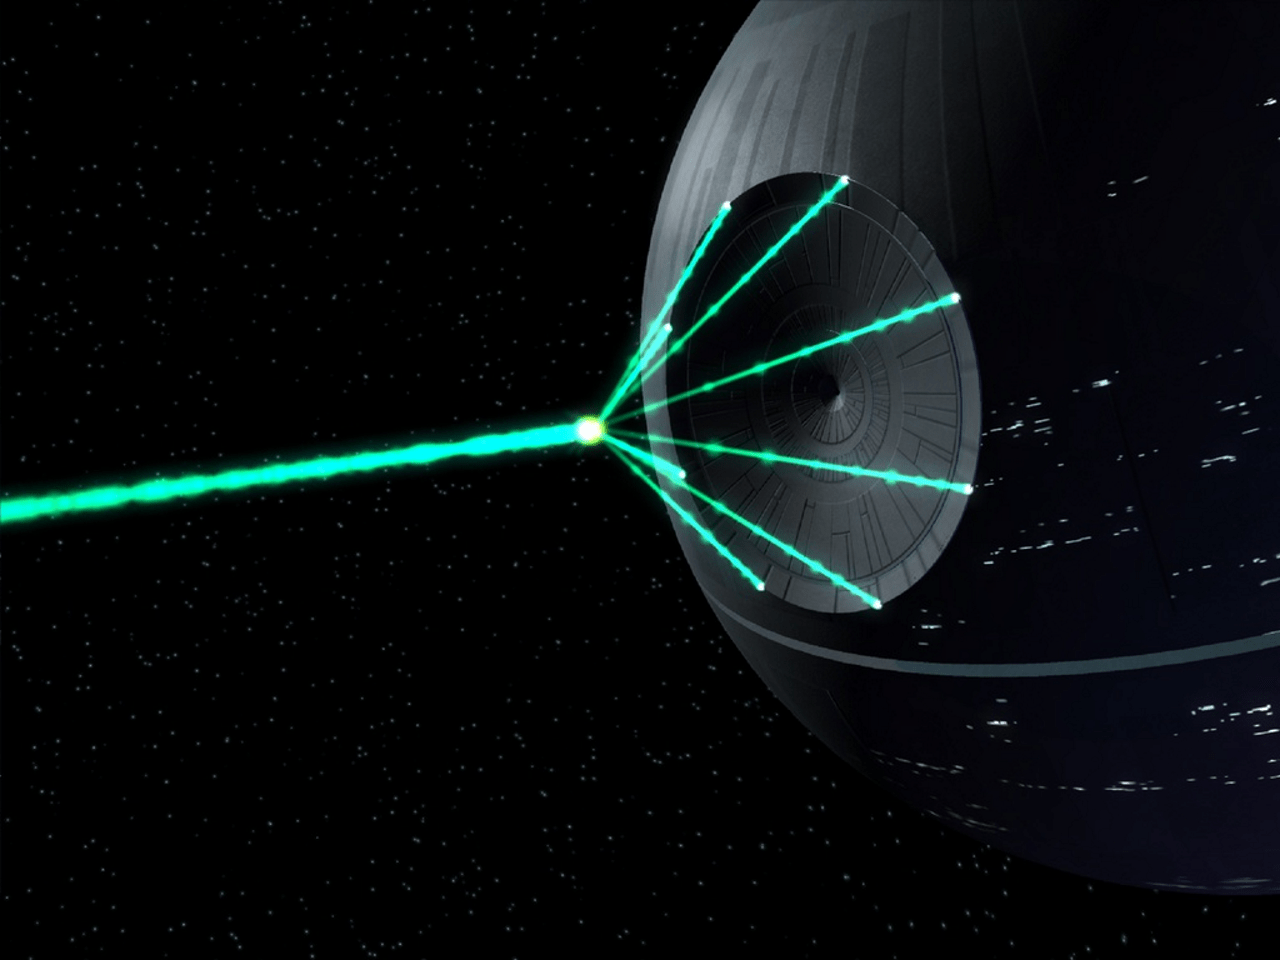
\includegraphics[height=6cm,width=1\textwidth,keepaspectratio]{deathstar.png}
            \caption*{Death Star --- Elliptic paraboloid}
            \label{fig:deathstar.png}
        \end{subfigure}
        \begin{subfigure}{0.32\textwidth}
            \href{https://www.youtube.com/watch?v=DiDU9b6BFLI}{
                \centering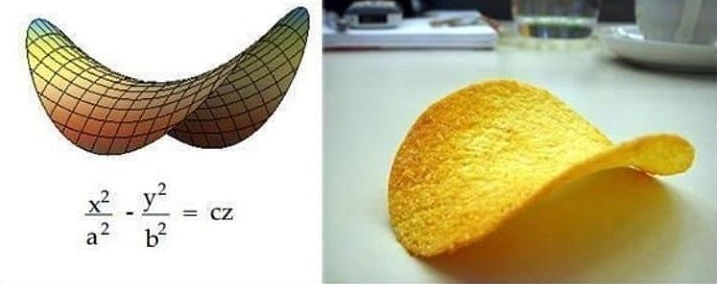
\includegraphics[height=6cm,width=1\textwidth,keepaspectratio]{pringles.jpg}}
            \caption*{Pringles --- Hyperbolic paraboloid}
            \label{fig:pringles.jpg}
        \end{subfigure}
        \begin{subfigure}{0.32\textwidth}
            \centering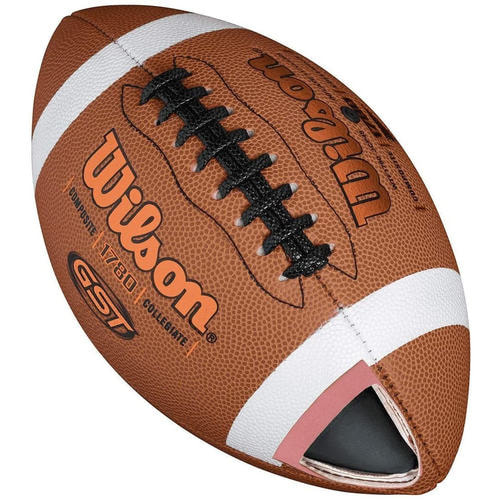
\includegraphics[height=6cm,width=1\textwidth,keepaspectratio]{rugby.jpg}
            \caption*{Rugby ball --- Ellipsoid}
            \label{fig:rugby.rugby}
        \end{subfigure}
    \end{figure}
\end{frame}

\begin{frame}[t]{How to determine a type of surface (\href{https://youtu.be/aM-0-oAppp0}{Video explanation})}
\framesubtitle{}
\vspace{-0.6cm}
\begin{figure}[H]
    \begin{subfigure}[t]{0.32\textwidth}
        \uncover<2->{\centering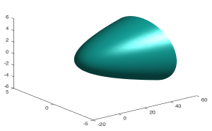
\includegraphics[height=2.3cm,width=1\textwidth,keepaspectratio]{1_1.png}}
        \caption{$2z^2+3y^2-x=1$ \\ \uncover<2->{Elliptic paraboloid}}
        \label{fig:1_1.png}
    \end{subfigure}
    \begin{subfigure}[t]{0.32\textwidth}
        \uncover<3->{\centering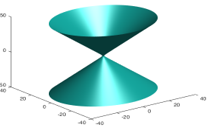
\includegraphics[height=2.3cm,width=1\textwidth,keepaspectratio]{1_2.png}}
        \caption{$2x^2+3y^2-z^2=1$ \\ \uncover<3->{Hyperboloid of one sheet}}
        \label{fig:1_2.png}
    \end{subfigure}
    \begin{subfigure}[t]{0.32\textwidth}
        \uncover<4->{\centering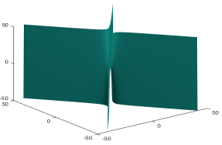
\includegraphics[height=2.3cm,width=1\textwidth,keepaspectratio]{1_3.png}}
        \caption{$-3x^2+2y^2-z=0$ \\ \uncover<4->{Hyperbolic paraboloid}}
        \label{fig:1_3.png}
    \end{subfigure}
\vspace{-0.3cm}

    \begin{subfigure}[t]{0.32\textwidth}
        \uncover<5->{\centering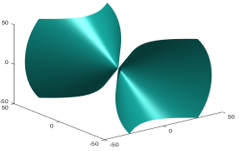
\includegraphics[height=2.3cm,width=1\textwidth,keepaspectratio]{1_4.png}}
        \caption{$-3x^2+2y^2-z^2=1$ \\ \uncover<5->{Hyperboloid of two sheets}}
        \label{fig:1_4.png}
    \end{subfigure}
    \begin{subfigure}[t]{0.32\textwidth}
        \uncover<6->{\centering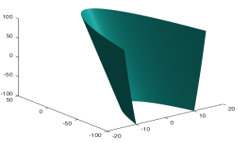
\includegraphics[height=2.3cm,width=1\textwidth,keepaspectratio]{1_5.png}}
        \caption{$2x^2+3y-z=0$ \\ \uncover<6->{Parabolic cylinder}}
        \label{fig:1_5.png}
    \end{subfigure}
    \begin{subfigure}[t]{0.32\textwidth}
        \uncover<7->{\centering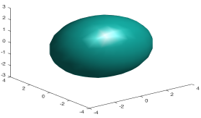
\includegraphics[height=2.3cm,width=1\textwidth,keepaspectratio]{1_6.png}}
        \caption{$2x^2+3y^2+4z^2=24$ \\ \uncover<7->{Ellipsoid}}
        \label{fig:1_6.png}
    \end{subfigure}
\end{figure}
\end{frame}

\begin{frame}[t]{How to sketch surfaces}
    \framesubtitle{Video}
    \vspace{-0.6cm}
    \begin{figure}[H]
        \href{https://youtu.be/UWbEd-9yfD0}{
            \centering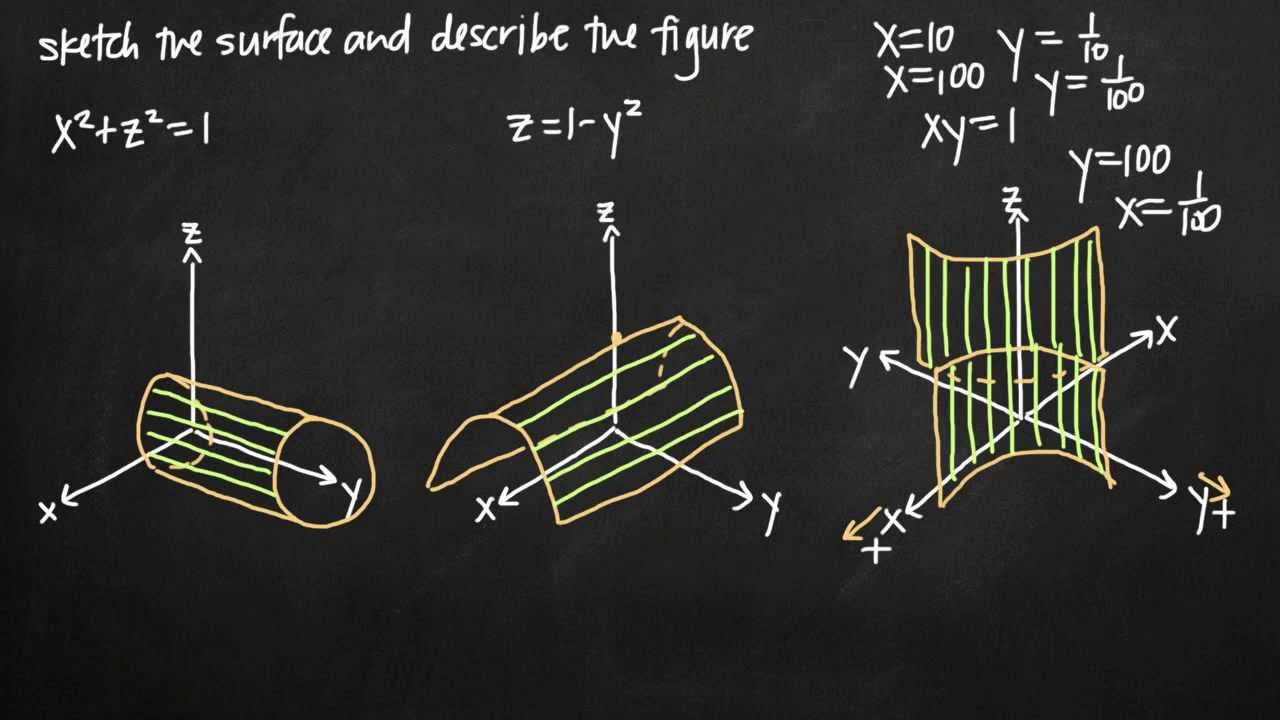
\includegraphics[height=6cm,width=1\textwidth,keepaspectratio]{sketch.jpg}}
        % \caption{Click on a picture for a video}
        \label{fig:sketch.jpg}
    \end{figure}
\end{frame}

\begin{frame}[t]{Case studies of 2nd order curve equation (ENG)}
\framesubtitle{}
    \vspace{-0.6cm}
    \begin{figure}[H]
        \centering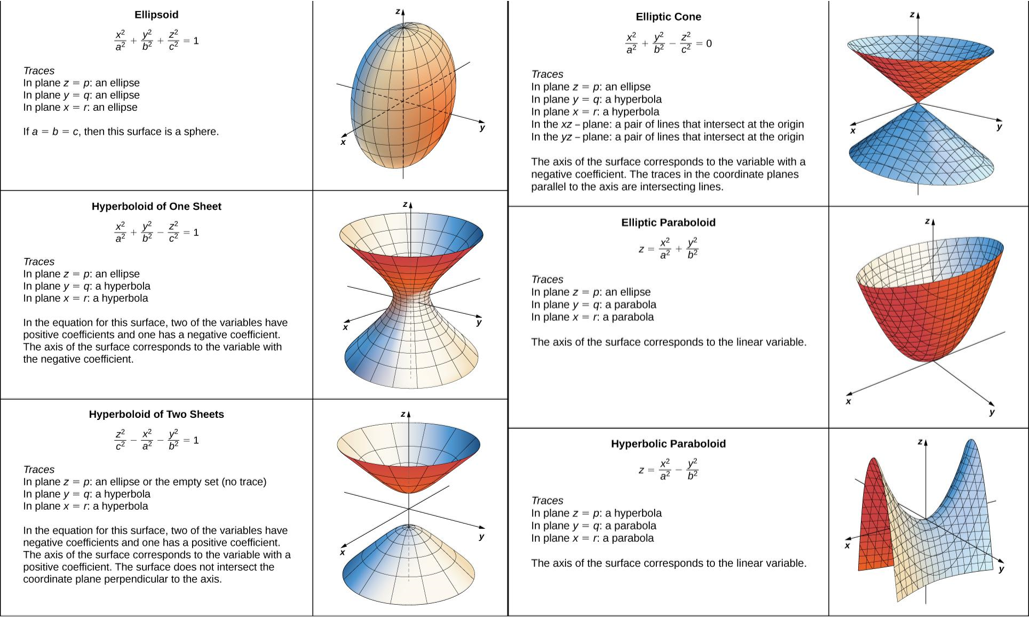
\includegraphics[height=6cm,width=1\textwidth,keepaspectratio]{curve_eq_eng.png}
        \label{fig:curve_eq_eng.png}
    \end{figure}
\end{frame}

\begin{frame}[t]{Case studies of 2nd order curve equation (RUS)}
    \framesubtitle{}
        \vspace{-0.6cm}
        \begin{figure}[H]
            \centering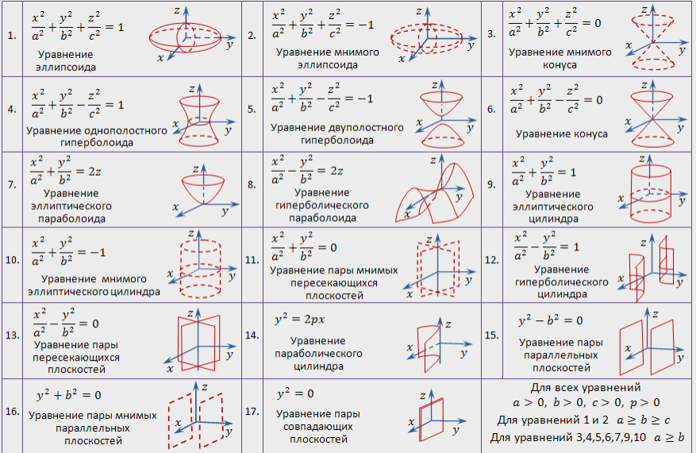
\includegraphics[height=6cm,width=1\textwidth,keepaspectratio]{curve_eq_rus.png}
            \label{fig:curve_eq_rus.png}
        \end{figure}
    \end{frame}

\begin{frame}[t]{Task 1}
    \framesubtitle{}
    \only<1>{
        Sketch the following surfaces:
        \begin{enumerate}
          \item $4-4y^2-z^2=x$
          \item $-x^2-y^2+z^2=1$
          \item $x^2+y^2-z^2=4$
        \end{enumerate}}
    \only<2>{
        \alert{\Large Answer for $4-4y^2-z^2=x$}
        \begin{figure}[H]
            \centering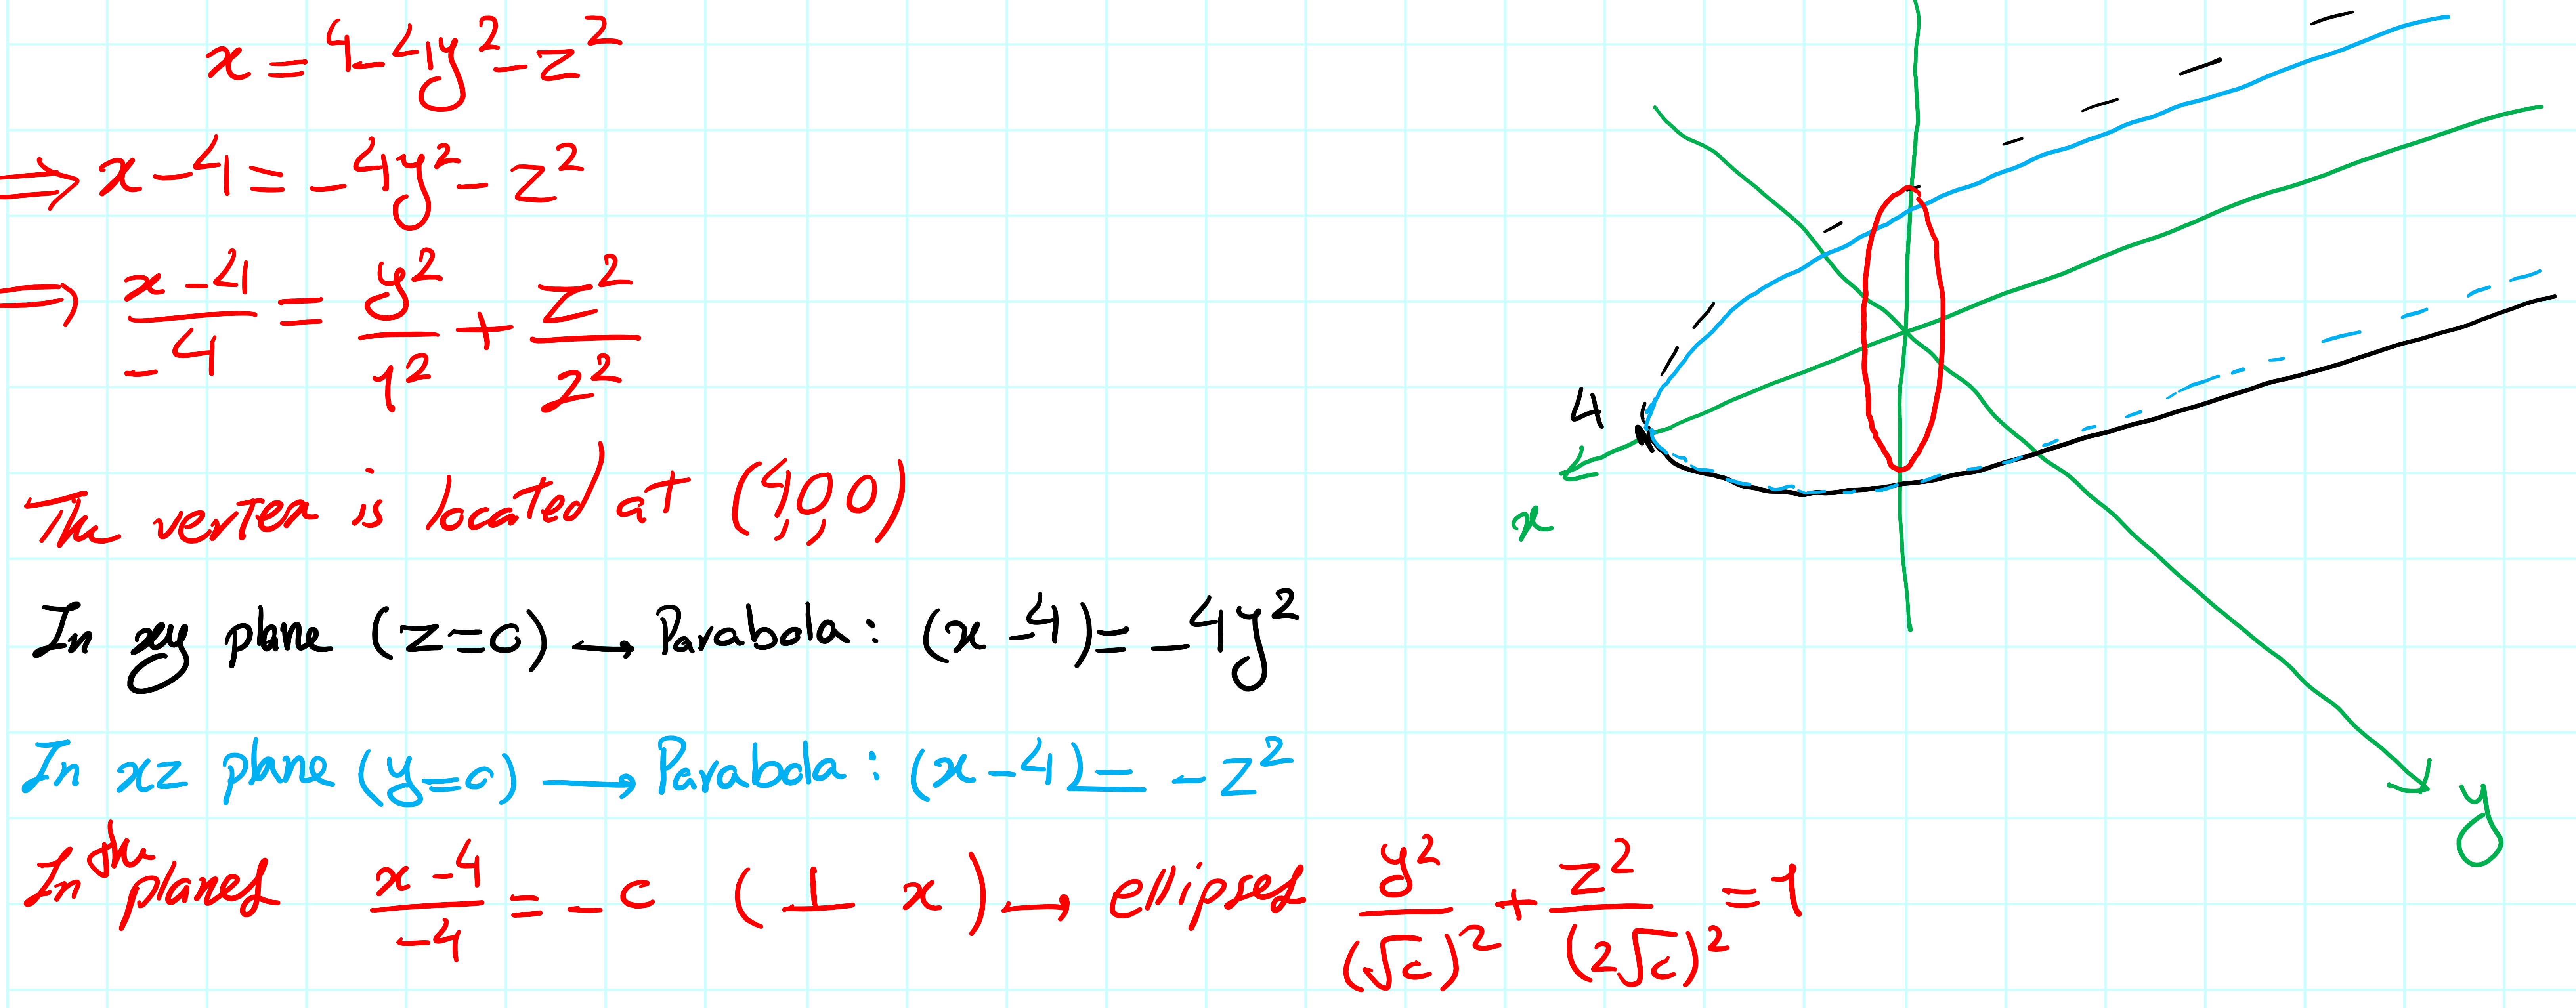
\includegraphics[height=5.5cm,width=1\textwidth,keepaspectratio]{1ans_1.png}
            % \caption{caption_name}
            \label{fig:1ans_1.png}
        \end{figure}
    }
    \only<3>{
        \alert{\Large Answer for $-x^2-y^2+z^2=1$}
        \begin{figure}[H]
            \centering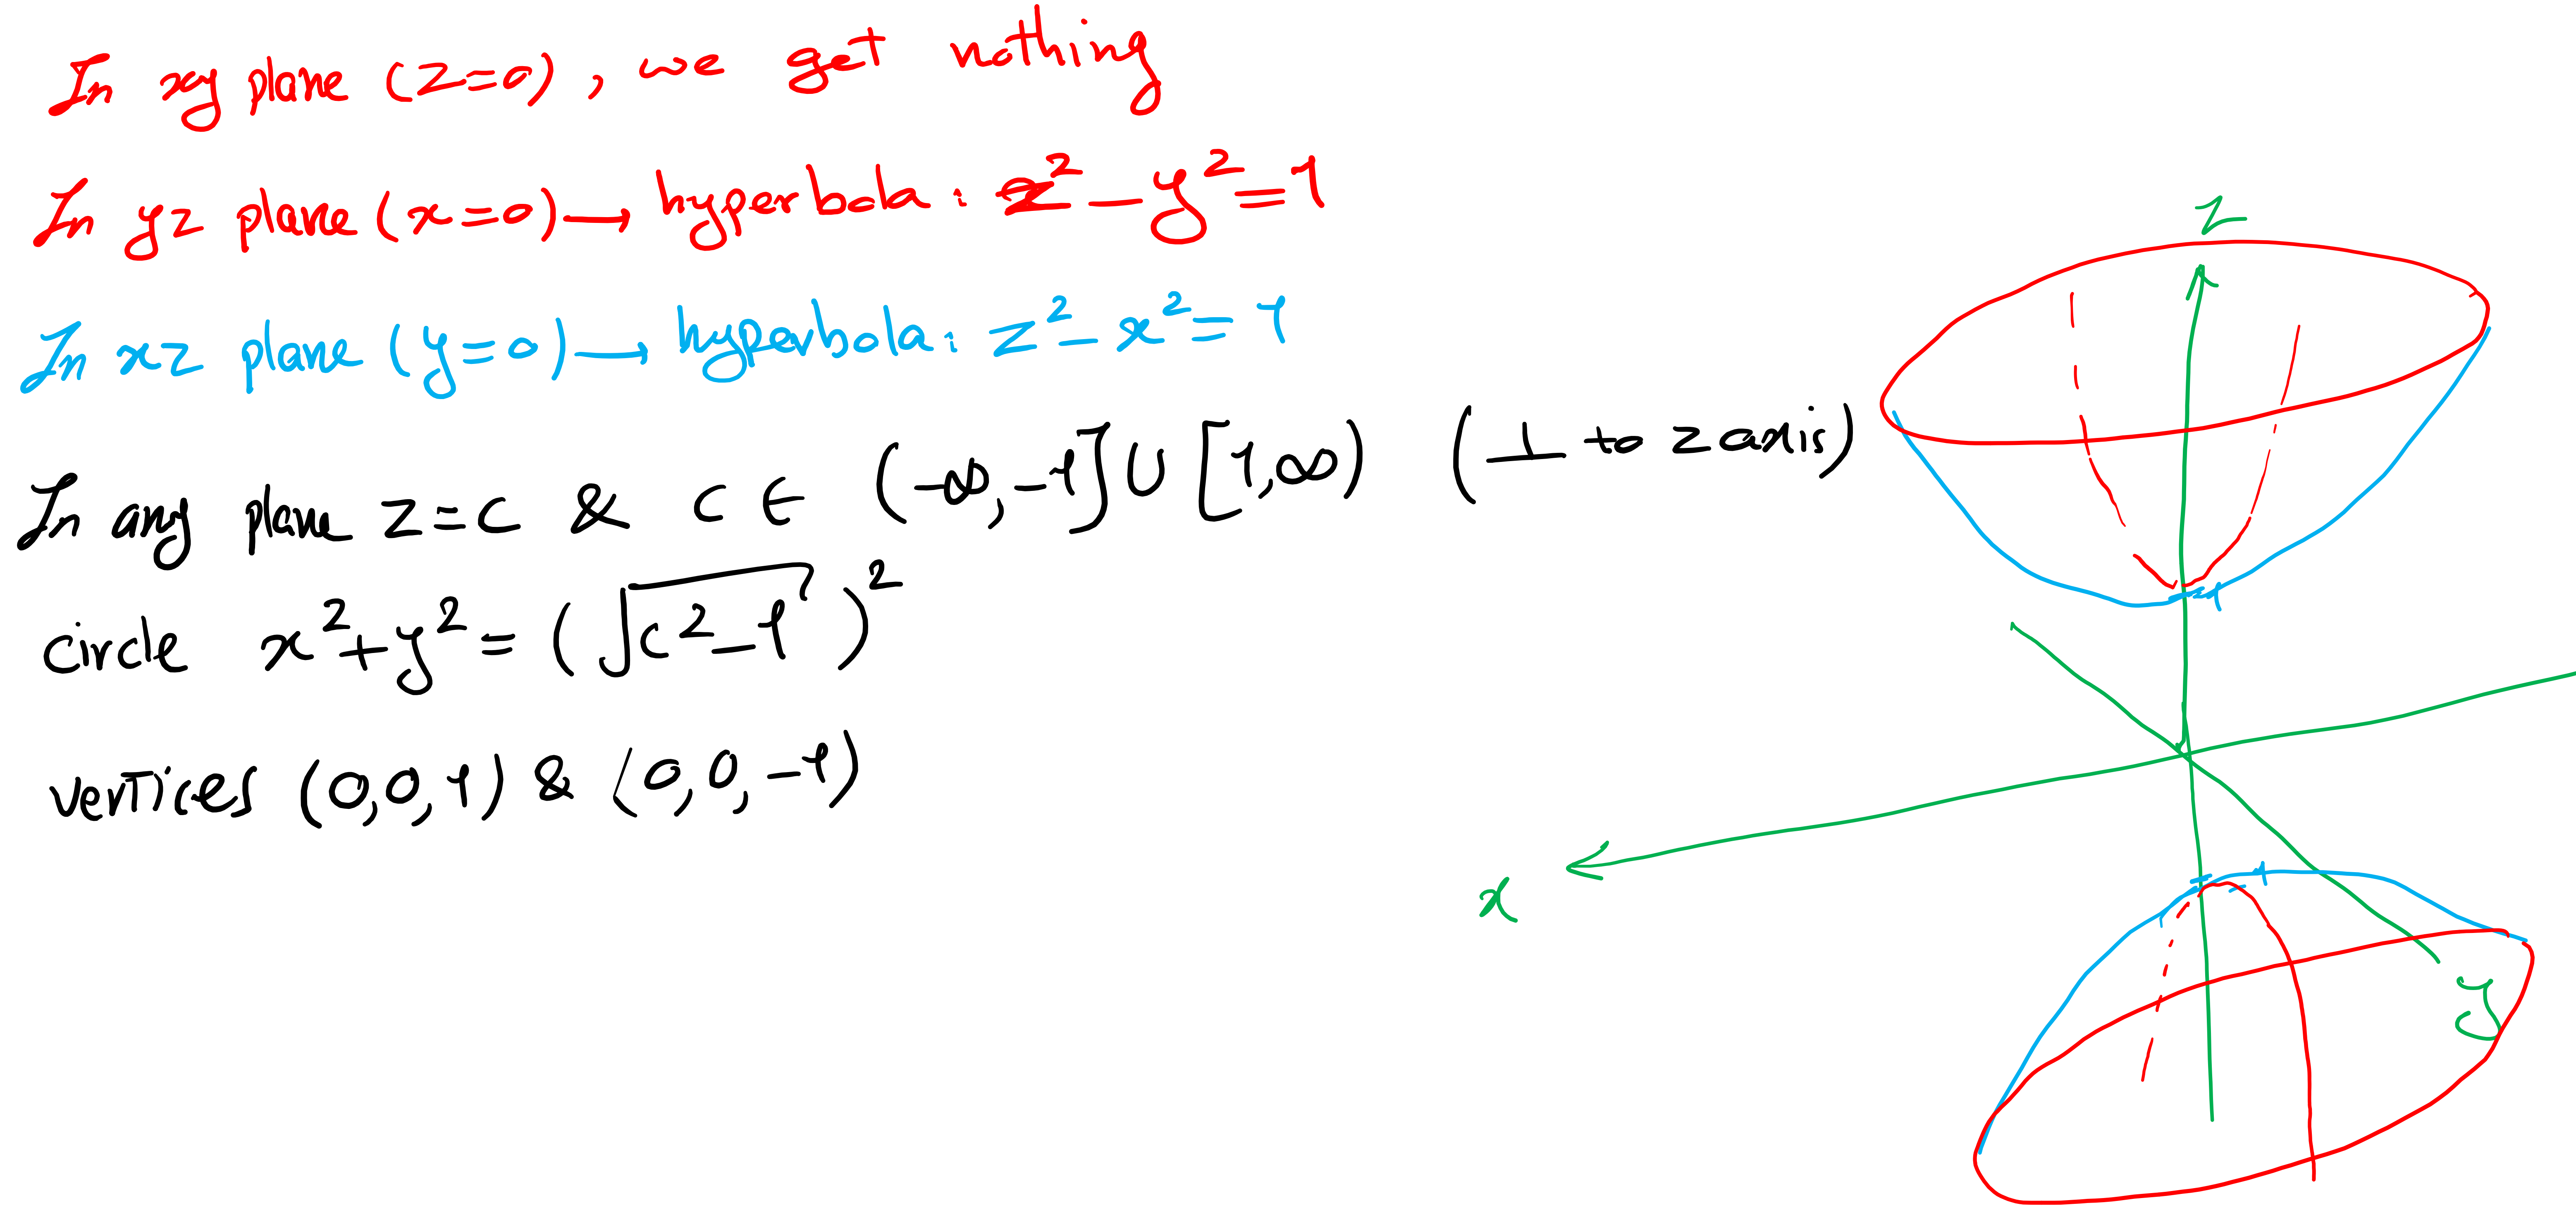
\includegraphics[height=5.5cm,width=1\textwidth,keepaspectratio]{1ans_2.png}
            % \caption{caption_name}
            \label{fig:1ans_2.png}
        \end{figure}
    }
    \only<4>{
        \alert{\Large Answer for $x^2+y^2-z^2=4$}
        \begin{figure}[H]
            \centering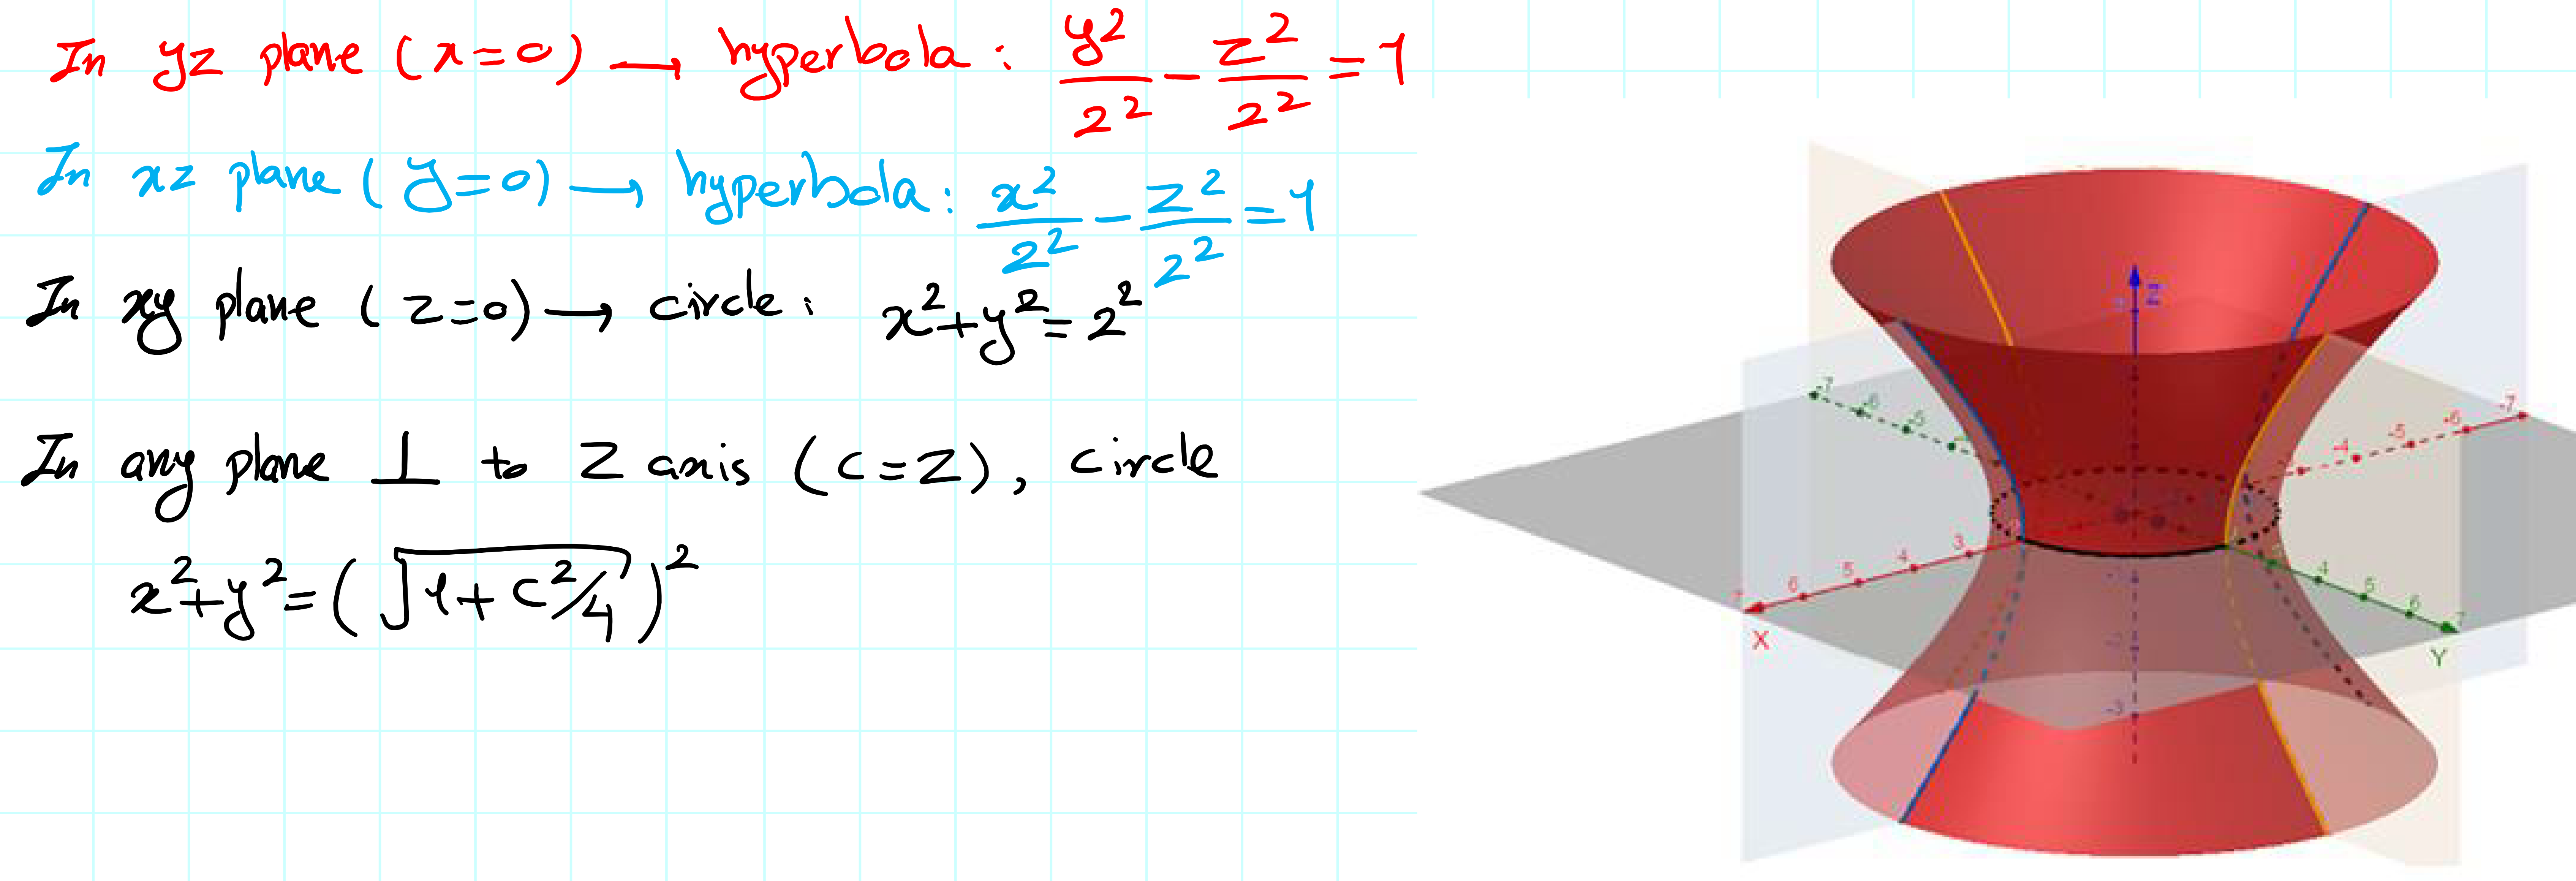
\includegraphics[height=5.5cm,width=1\textwidth,keepaspectratio]{1ans_3.png}
            % \caption{caption_name}
            \label{fig:1ans_3.png}
        \end{figure}
    }
\end{frame}

\begin{frame}[t]{Task 2}
    \framesubtitle{}
    \only<1>{
        Find the equation of the sphere which passes through the points $(2, 7, -4)$ and $(4, 5, -1)$ has its centre on the line joining these two points as diameter. }
    \only<2>{
        \alert{\Large Answer}
        \begin{figure}[H]
            \centering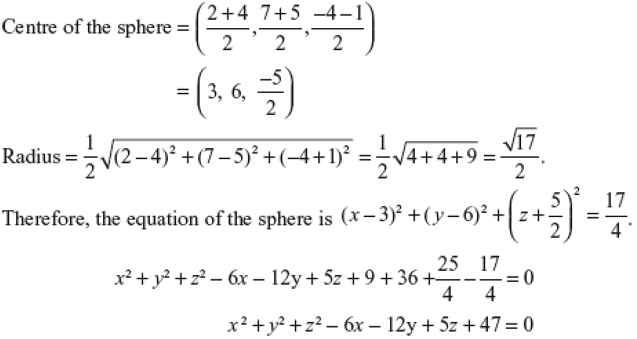
\includegraphics[height=5.5cm,width=1\textwidth,keepaspectratio]{2ans.png}
            % \caption{caption_name}
            \label{fig:2ans.png}
        \end{figure}
    }
\end{frame}

\begin{frame}[t]{Task 3}
    \framesubtitle{}
    \only<1>{
        Find the equation of the sphere which touches the coordinate axes, whose centre lies in the positive octant and has a radius 4. }
    \only<2>{
            \vspace{-0.6cm}
            \begin{figure}[H]
                \href{https://www.geogebra.org/calculator/t4hqsuvm}{
                    \centering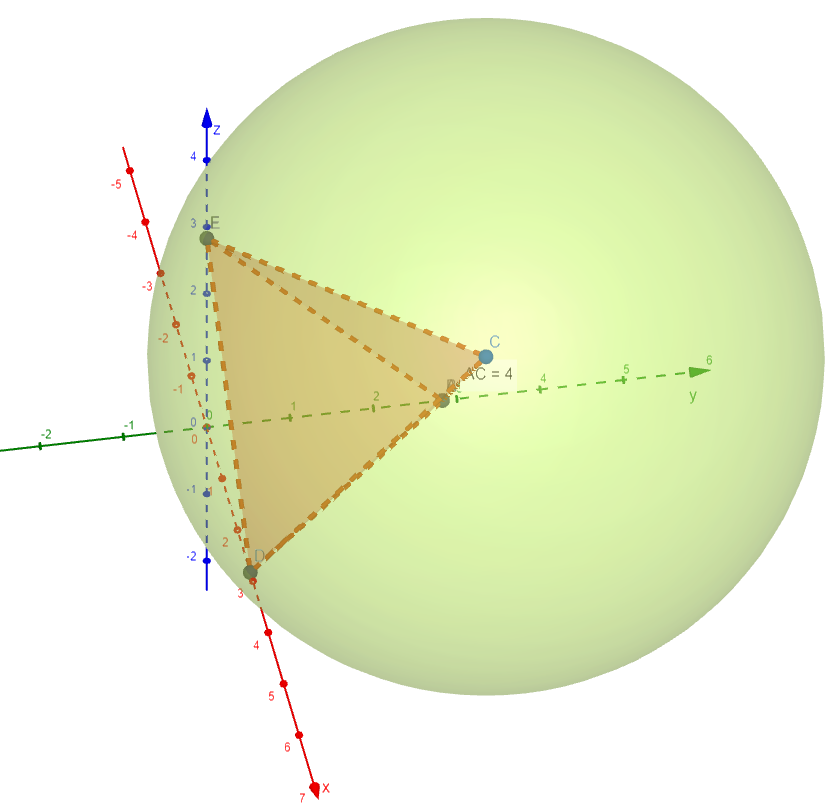
\includegraphics[height=6cm,width=1\textwidth,keepaspectratio]{3ans_1.png}}
                \label{fig:file_name}
            \end{figure}
    }
    \only<3>{
        \alert{\Large Answer}
        \begin{figure}[H]
            \centering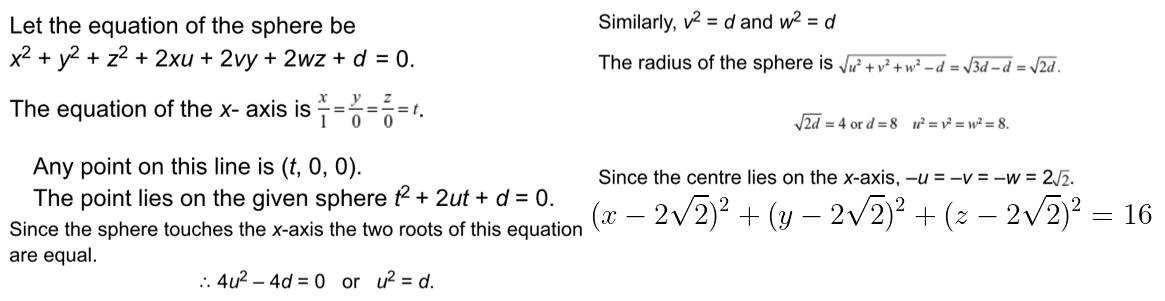
\includegraphics[height=5.5cm,width=1\textwidth,keepaspectratio]{3ans.png}
            % \caption{caption_name}
            \label{fig:3ans.png}
        \end{figure}
    }
\end{frame}

\begin{frame}[t]{Task 4}
    \framesubtitle{}
    \only<1>{
        Show that the plane $4x - 3y + 6z - 35 = 0$ is a tangent plane to the sphere $x^2 + y^2 + z^2 - y - 2z - 14 = 0$ and find the point of contact. }
    \only<2>{
        \alert{\Large Answer}
        \begin{figure}[H]
            \centering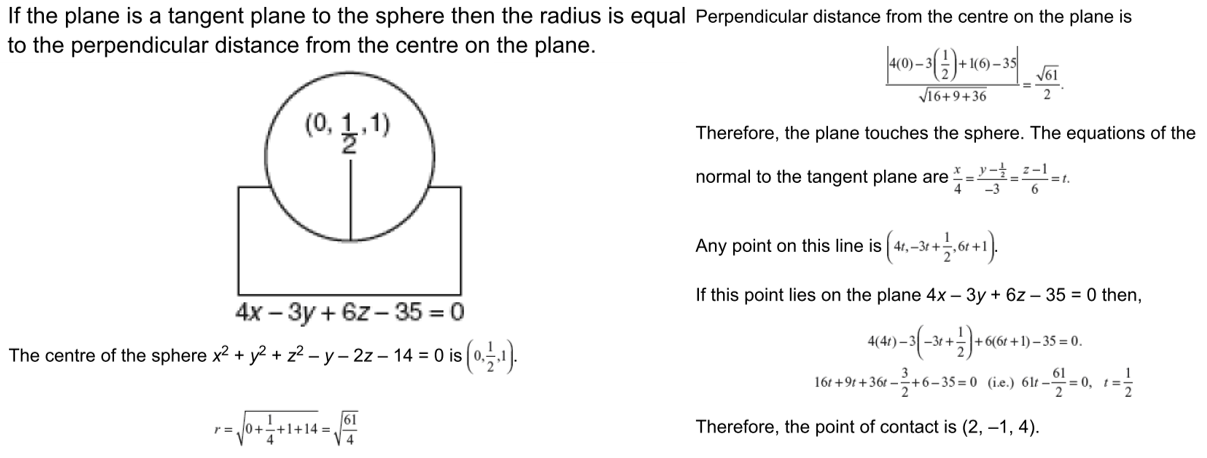
\includegraphics[height=5.5cm,width=1\textwidth,keepaspectratio]{4ans.png}
            % \caption{caption_name}
            \label{fig:4ans.png}
        \end{figure}
    }
\end{frame}

\begin{frame}[t]{Task 5}
    \framesubtitle{}
    \only<1>{
        Obtain the equations to the sphere through the common circle of the sphere $x^2 + y^2 + z^2 + 2x + 2y = 0$ and the plane $x + y + z + 4 = 0$ which intersects the plane $x + y = 0$ in circle of radius 3 units.}
    \only<2>{
        \alert{\Large Answer}
        \begin{columns}[T,onlytextwidth]
            \begin{column}{0.49\textwidth}
                \begin{figure}[H]
                    \centering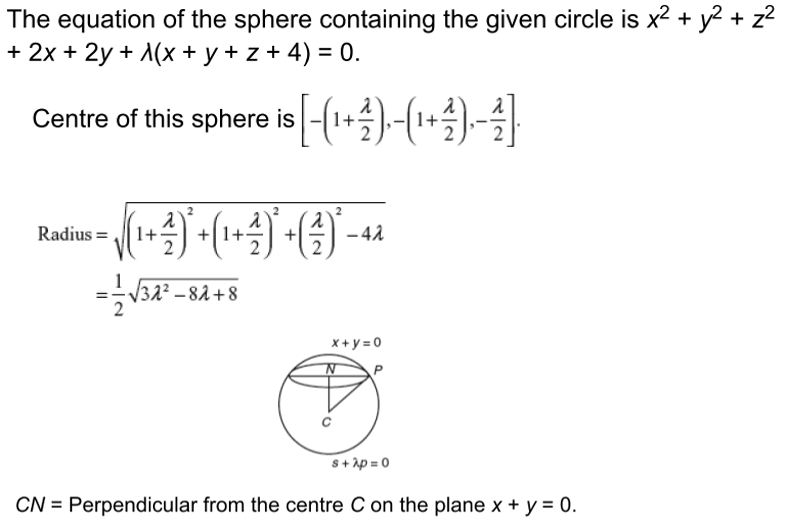
\includegraphics[height=6cm,width=1\textwidth,keepaspectratio]{5ans_1.png}
                    % \caption{caption_name}
                    \label{fig:5ans_1.png}
                \end{figure} 
            \end{column}
            \begin{column}{0.49\textwidth}
                \vspace{-2cm}
                \begin{figure}[H]
                    \href{https://www.geogebra.org/calculator/tfne7h58}{
                        \centering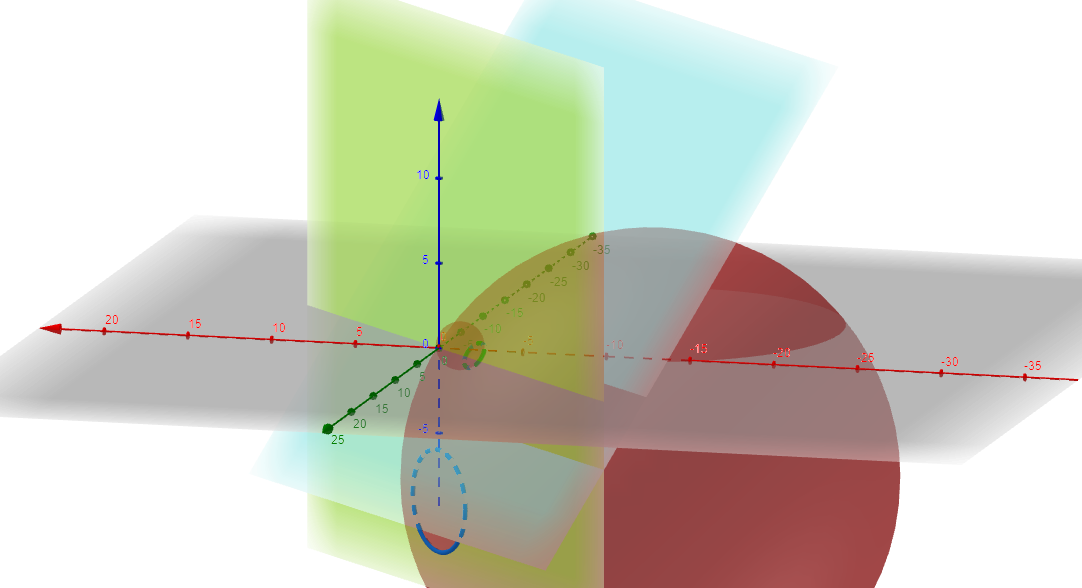
\includegraphics[height=2.5cm,width=1\textwidth,keepaspectratio]{5ans_2.png}}
                    % \caption{caption_name}
                    \label{fig:5ans_2.png}
                \end{figure}
                \begin{figure}[H]
                    \centering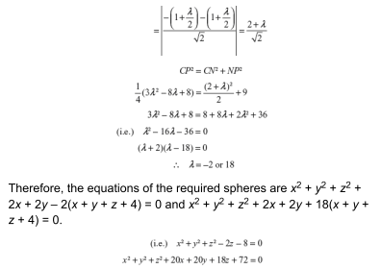
\includegraphics[height=3.5cm,width=1\textwidth,keepaspectratio]{5ans_3.png}
                    % \caption{caption_name}
                    \label{fig:5ans_3.png}
                \end{figure}
            \end{column}
        \end{columns}

    }
\end{frame}

\begin{frame}[t]{Task 6}
    \framesubtitle{}
    \only<1>{
        Find the equation of the sphere which touches the plane $3x + 2y - z + 2 = 0$ at the point $(1, -2, 1)$ and cuts orthogonally the sphere $x^2 + y^2 + z^2 - 4x + 6y + 4 = 0$
        \begin{figure}[H]
            \centering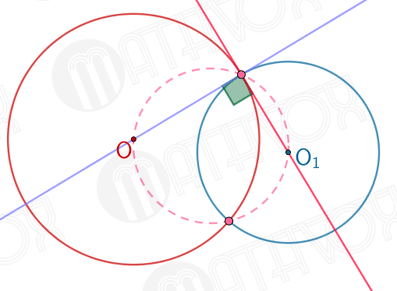
\includegraphics[height=4cm,width=1\textwidth,keepaspectratio]{cut_orhogonally.png}
            \caption*{Orthogonal circles}
            \label{fig:cut_orhogonally.png}
        \end{figure}
    }
    \only<2>{
            \vspace{-0.6cm}
            \begin{figure}[H]
                \href{https://www.geogebra.org/calculator/gdt9r9rx}{
                    \centering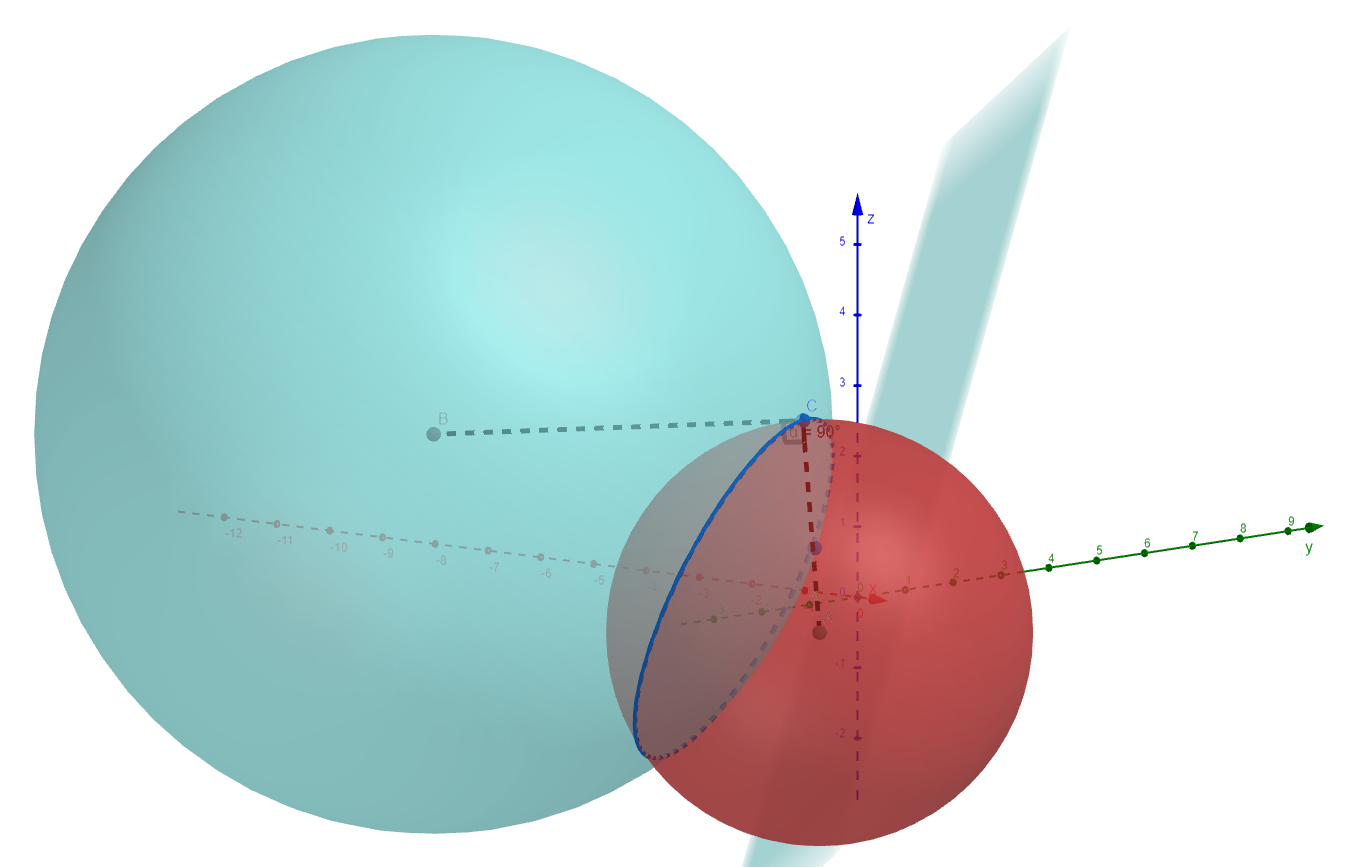
\includegraphics[height=6cm,width=1\textwidth,keepaspectratio]{6ans_1.png}}
                \label{fig:file_name}
            \end{figure}
    }
        \only<3>{
        \alert{\Large Answer}
        \begin{figure}[H]
            \centering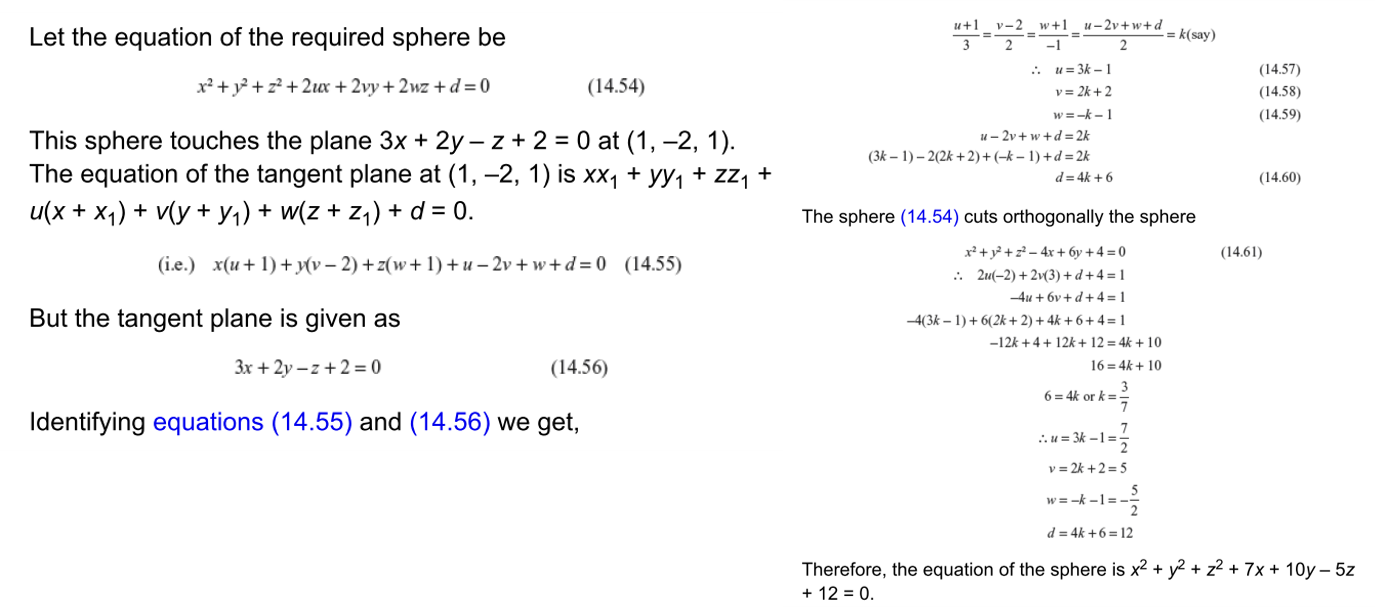
\includegraphics[height=5.5cm,width=1\textwidth,keepaspectratio]{6ans.png}
            % \caption{caption_name}
            \label{fig:6ans.png}
        \end{figure}
    }
\end{frame}



\begin{frame}[t]{Reference material}
    \Large
    \begin{itemize}
        \item \href{http://www.mathprofi.ru/poverhnosti.html}{How to sketch surfaces (Mathprofi, rus)}
        \item \href{https://youtu.be/DbpieqgKKRM}{Reducing a quadric surface equation to standard form (video, eng)}
    \end{itemize}
\end{frame}

\fbckg{fibeamer/figs/last_page.png}
\frame[plain]{}

\end{document}